\chapter{Evaluation}
We evaluate our method based on the development data set from the ChAirGest
corpus~\cite{Ruffieux2013} with gestures captured from 10 users. There are 900
total gesture occurrences (3 recording sessions for each user) in the
development data set representing three forth of the entire corpus. The remaining one forth of the corpus are not released to
the public, and can be used for final evaluation on unseen data.

In this data set, on average, the hand is at 1.2m away
from the sensor, which means the depth error is around 5mm.

\begin{table}[h]
\begin{center}
\begin{tabular}{|l|p{2cm}|p{1.7cm}|p{1.7cm}|}
\hline
 & Hand position from salience detection \& Xsens & Hand position
 from Kinect skeleton \& Xsens & Xsens Only \\
\hline
F1 Score & \textbf{0.907 (0.01)} & 0.870 (0.02) & 0.890 (0.02) \\
\hline
ATSR Score & \textbf{0.923 (0.02)} & 0.930 (0.03) & 0.920 (0.01) \\
\hline
Final Score & \textbf{0.912 (0.01)} & 0.881 (0.01) & 0.895 (0.01) \\
\hline
\end{tabular}
\caption{Comparison of the average 3-fold cross validation results for different
feature vectors. Values in parentheses are standard deviations.}
\label{tab:comp-feature}
\end{center}
\end{table}

\begin{table}[h]
\begin{center}
\begin{tabular}{|l|p{2cm}|p{1.7cm}|p{1.7cm}|}
\hline
 & color & depth & both \\
\hline
F1 Score & 0.703 (0.01) & 0.720 (0.02) & 0.723 (0.01) \\
\hline
ATSR Score & 0.870 (0.01) & 0.880 (0.01) & 0.873 (0.01) \\
\hline
Final Score & 0.732 (0.01) & 0.748 (0.01) & 0.749 (0.00) \\
\hline
\end{tabular}
\caption{Comparison of the average 3-fold cross validation results for
features from color and depth sensors. Values in parentheses are standard
deviations.}
\label{tab:comp-feature}
\end{center}
\end{table}

\begin{figure}[h]
\centering
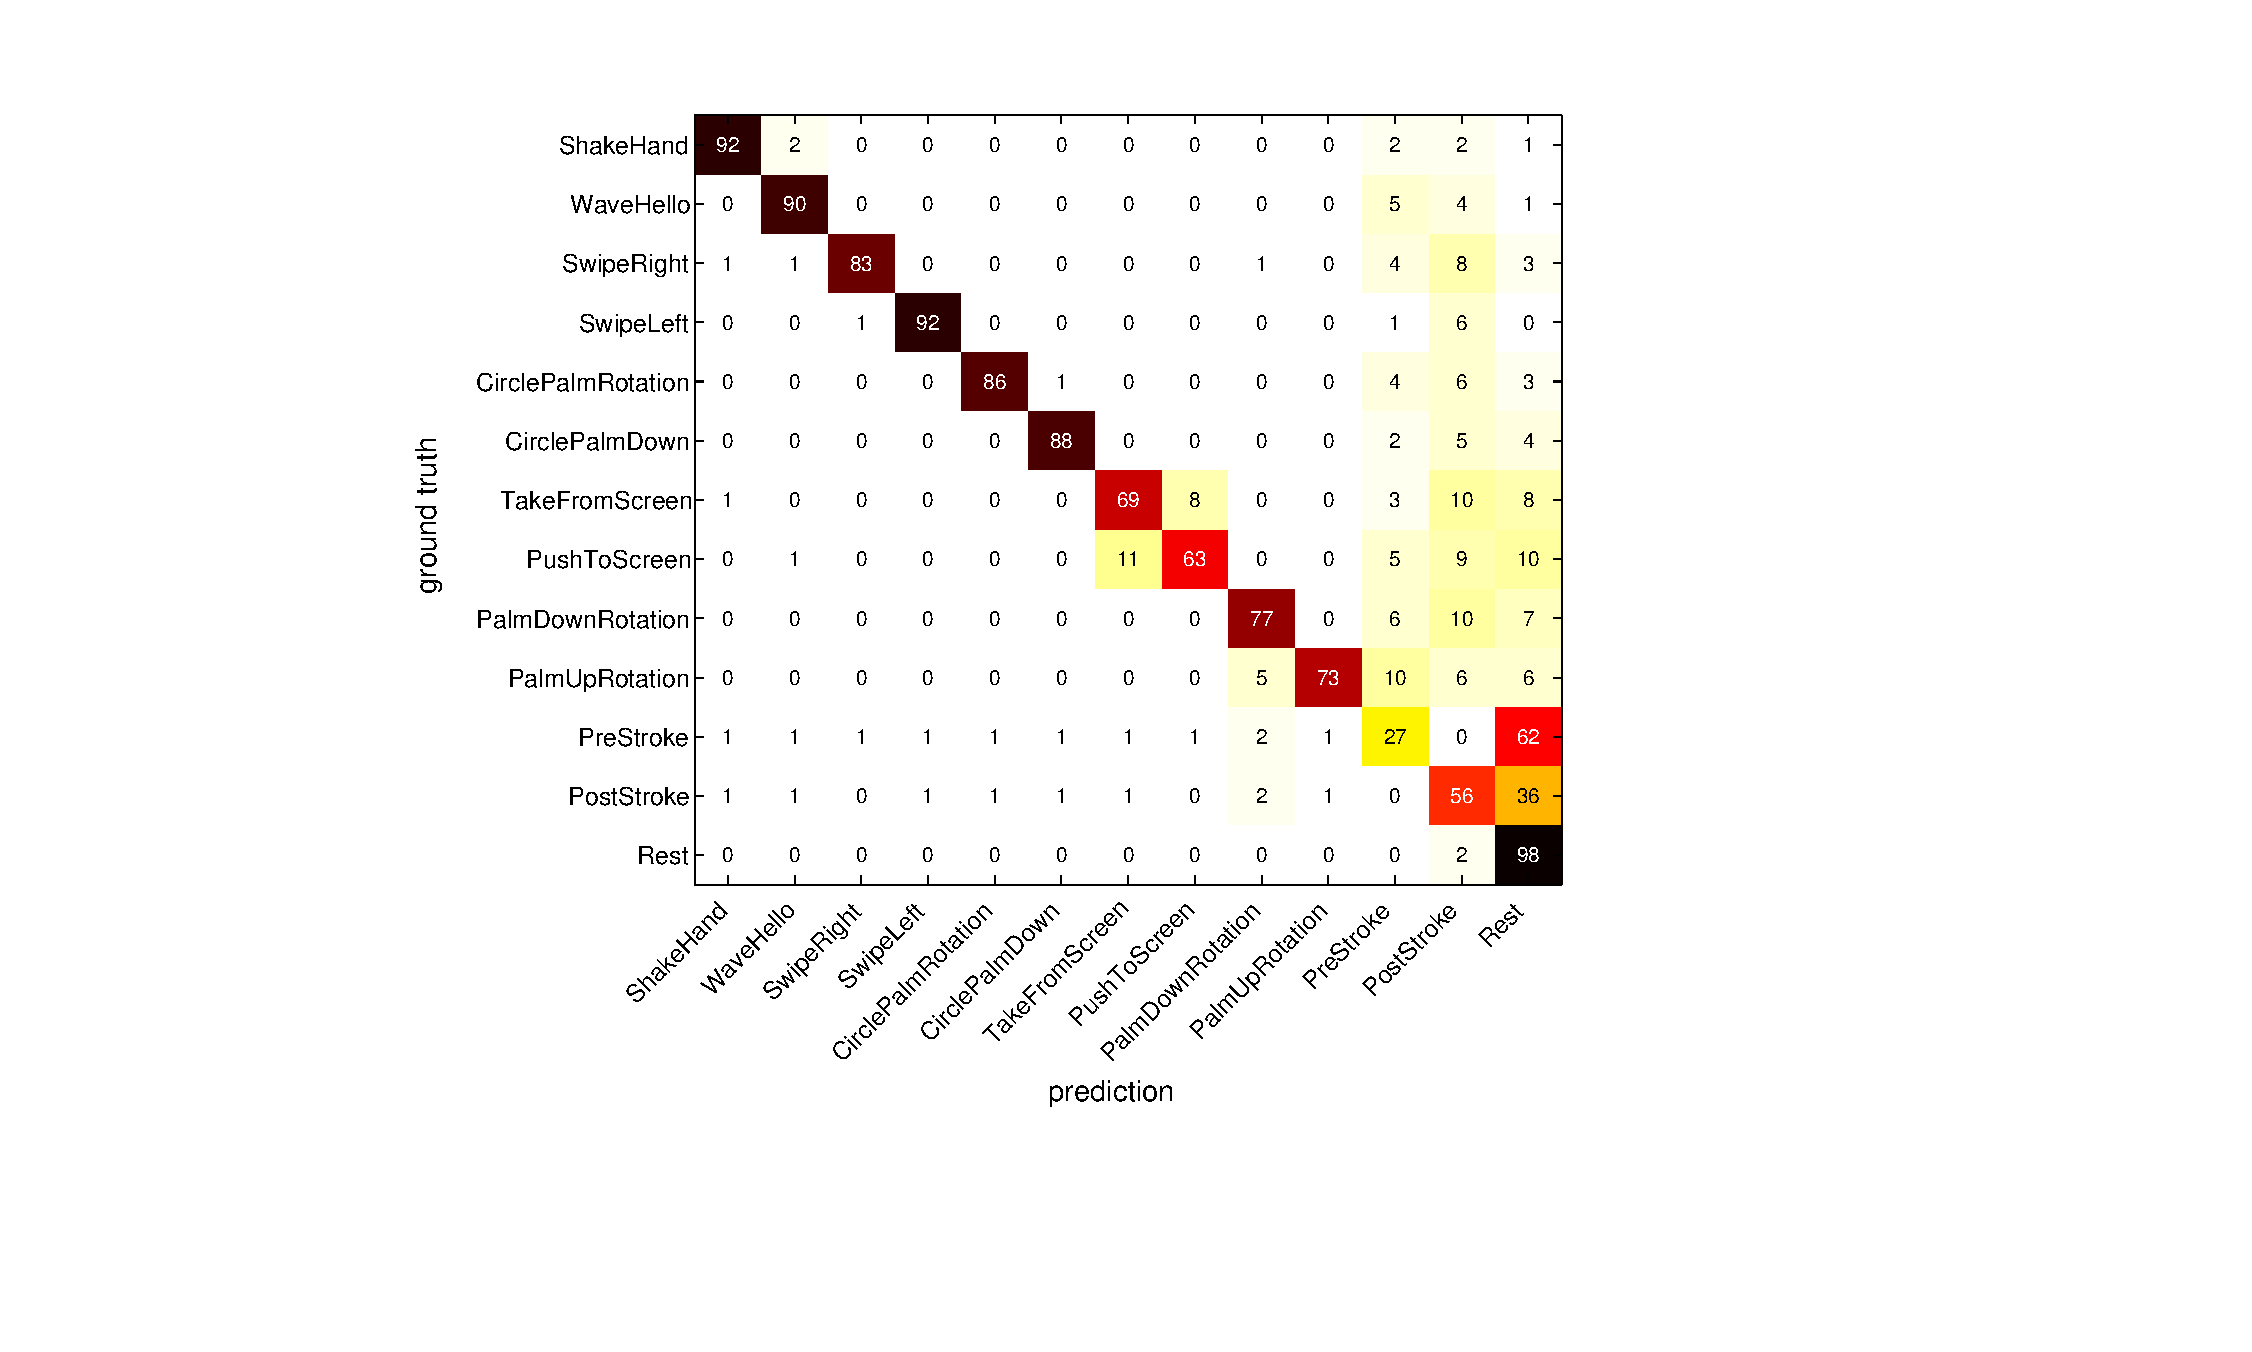
\includegraphics[trim={6cm 3.5cm 10cm 1.5cm}, clip,
width=1\columnwidth]{figures/confusion-matrix.eps} \caption{Per frame
classification confusion matrix based on result from 3-fold cross validation using both Kinect and Xsens features. The numbers are percentages. The darker the color the higher the percentage.}
\label{fig:confusion}
\end{figure}

\begin{figure}[tb]
\centering
\includegraphics[trim={6cm 3.5cm 10cm 1.5cm}, clip,
width=1\columnwidth]{figures/confusion_color_depth.png} \caption{Per frame
classification confusion matrix based on result from 3-fold cross validation using 
both color and depth images for hand. The numbers are percentages. The darker
the color the higher the percentage.}
\label{fig:confusion}
\end{figure}

``Take from Screen'' and ``Push to Screen'' have the lowest recognition
accuracy, especially when using the kienct data. We notice that when the users
extend their hands towards the screen, the hands are too close to the sensor
(below the too near range), and the depth sensor cannot get accurate readings.

